%%%%%%%%%%%%%%%%%%%%% chapter.tex %%%%%%%%%%%%%%%%%%%%%%%%%%%%%%%%%
%
% sample chapter
%
% Use this file as a template for your own input.
%
%%%%%%%%%%%%%%%%%%%%%%%% Springer-Verlag %%%%%%%%%%%%%%%%%%%%%%%%%%
%\motto{Use the template \emph{chapter.tex} to style the various elements of your chapter content.}
\chapter{Cut \& Count für Steiner Tree}
\label{c:cc_steiner}

\section{Steiner Tree}
\label{sec:steiner}
\begin{definition}
Steiner Tree\\
\textbf{Input}: An undirected graph $G = (V, E)$, a set of terminals $T \subseteq V$ and an integer $k$. \\
\textbf{Question}: Is there a set $X \subseteq V$ of cardinality $k$ such that $T \subseteq X$ and $G[X]$ is connected?
\end{definition}

Bei dem Steiner-Tree Problem handelt es sich um ein connectivity-Typ Problem. In einen gegebenen Graphen sind einige Knoten als Terminale makiert. Nun wird nach einem Subgraphen innerhalb des Ursprungsgraphen gesucht, der alle Terminale enthält und aus k vielen Knoten insgesamt besteht. Desweiteren müssen alle Knoten innerhalb des Subgraphen über Kanten untereinander erreichbar sein.

\section{Cut}
\label{sec:st_cut}
Zu beginn des Cut-Part wird eine zufällige Gewichtsfunktion $\omega:V\rightarrow \{1,\dots,N\}$ definiert. Diese wird für die Isolation der Lösungsmenge verwendet.\\
Desweiteren wird im Cut-Part die Menge $\mathcal{R}_W$ definiert. Sie ist die Menge aller Teilmengen von $X$ aus $V$ mit $T \subseteq X$, $\omega(X)=W$ und $|X|=k$. Somit stellt die Menge $\mathcal{R}_W$ die Menge aller Lösungskandidaten dar.\\
Eine weitere zu definierende Menge ist $\mathcal{S}_W=\{X \in \mathcal{R}_W | G[X]$ ist zusammenhängend$\}$. Somit bildet die Menge $\mathcal{S}_W$ Lösungen für ein gegebenes bestimmtes Gewicht $W$.\\
$\cup_W \mathcal{S}_W$ bildet so die Lösungsmenge. Gibt es nun ein Gewicht $W$ für das die Menge nicht leer ist, so gibt der Algorithmus eine positive Antwort.\\
Von der Menge der Terminalknoten wird ein Terminal als $v_1$-Terminal festgelegt. Dieses dient dazu, dass bei der Bildung von konsistenten Cuts keine Cuts doppelt gezählt werden.\\
Die konsistenten Cuts werden in der Menge  $\mathcal{C}_W$ beschrieben. Diese Bilden die Menge aller Subgraphen, die einen konsistenten Cut $(X,(X_1,X_2))$ bilden, wobei $X\in \mathcal{R}_W$ und $v_1 \in X_1$.
\begin{figure}
\label{fig:st_cut}
  \centering
    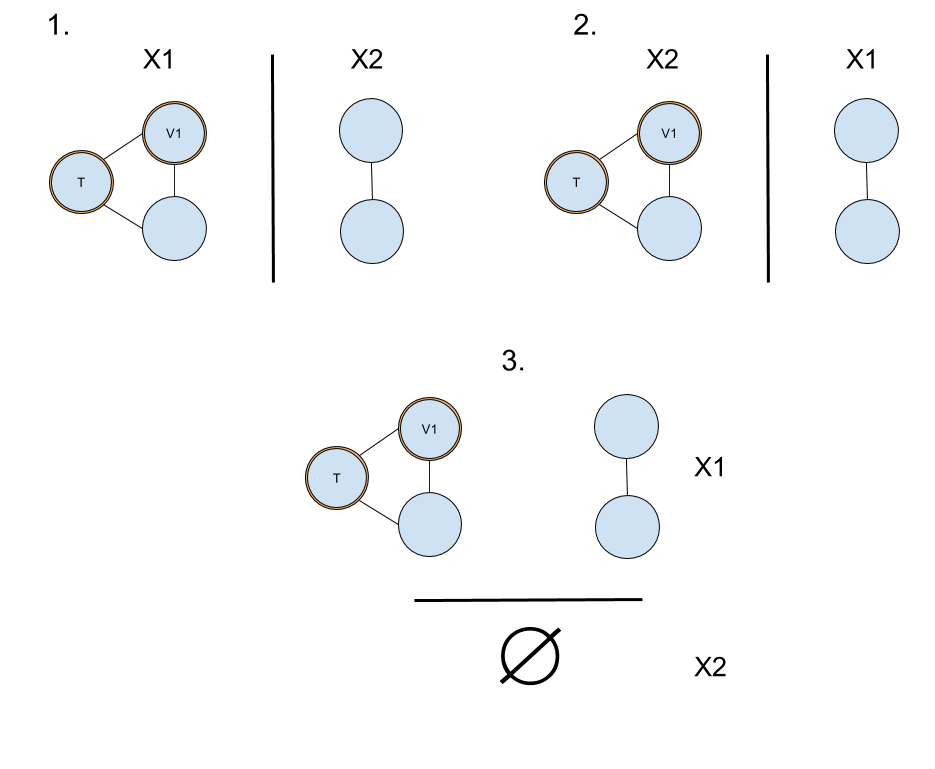
\includegraphics[width=1.0\textwidth]{./imgs/terminal_v1.png}
  	\caption{Konsistente Cuts ohne Beschränkung $v_1 \in X_1$. Man sieht, dass die konsistenten Cuts 1 und 2 identisch sind.}
\end{figure}

Die Anzahl der konstistenten Cuts sind im Lemma 3.3 des Papers beschrieben:\\
Let $G=(V,E)$ be a graph and let $X$ be a subset of vertices such that $v_1 \in X \subseteq V$. The number of consistently cut subgraphs $(X,(X_1,X_2))$ such that $v_1 \in X_1$ is equal to $2^{cc(G[X])-1}$.

Beweis: Per Definition ist bekannt, dass für jeden konsistenten Cut $(X,(X_1,X_2))$ und Connected Component $C$ aus $G[X]$ $C$ entweder in $X_1$ oder in $X_2$ enthalten sein muss. Für die Connected Component, die $v_1$ enthält ist die Wahl der Submenge fix. Für alle anderen Connected Components kann die Zugehörigkeit von Submengen frei gewählt werden. Daher erhalten wir $2^{cc(G[X])-1}$ verschiedene konsistente Cuts.

\section{Count}
\label{sec:st_count}
Aus Lemma 3.3 ist bekannt: $|\mathcal{C}|=\sum_{X \in \mathcal{R}} 2^{cc(G[X])-1}$. Wir legen $W$ fest und ignorieren die Indices: $|\mathcal{C}| \equiv |\{X \in \mathcal{R} |cc(G[X]) = 1\}| = |\mathcal{S}|$. In Worte gefasst bedeutet dies, dass die Anzahl der konsistenten Cuts eines Graphen modulo zwei gleich die Anzahl der Lösungen ist. Im Lemma 3.4 trifft das Paper dazu eine Aussage: Let $G,$ $\omega$, $\mathcal{C}_W$ and $\mathcal{S}_W$ be as defined above. Then for every $W$, $|\mathcal{S}_W| \equiv |\mathcal{C}_W|$.

\section{Dynamisches Programm}
\label{sec:dynP}

$|\mathcal{C}_W|$ modulo $2$ kann mit dynamischen Programm auf der NTD $\mathbb{T}$ berechnet werden.
für jeden Bag $x \in \mathbb{T}$, integers $0 \leq i \leq k,0 \leq w \leq kN$ und Färbung $s \in \{0,1_1,1_2 \}^{B_x}$ definiere:
\begin{itemize}
\item $\mathcal{R}_x(i,w)=\{X \subseteq V_x | (T \cap V_x) \subseteq X$ $\wedge$ $|X| = i$ $\wedge$ $\omega (X) = w \}$
\item $\mathcal{C}_x (i,w) =\{ (X,(X_1,X_2)) | X \in \mathcal{R}_x(i,w)$ $\wedge$ $(X,(X_1,X_2))$ is a consistently cut subgraph of $G_x$ $\wedge$ $(v_1 \in V_x \Rightarrow v_1 \in X_1 \} $
\item $\mathcal{A}_x(i,w,s)=| \{ (X,(X_1,X_2)) \in \mathcal{C}_x(i,w) | (s(v) = 1_j \Rightarrow v \in X_j)$ $\wedge$ $(s(v)=0 \Rightarrow v \notin X \} |$
\end{itemize}
Die Färbungen der Knoten gibt an ob sie zu einem konsistenten Cut gehören und wenn ja zu welcher der beiden Teilmengen des konsistenten Cuts sie gehören.
Färbung $s \in \{0,1_1,1_2 \}^{B_x}$  der Knoten aus $B_x$ bzgl. der Menge $C_x$
\begin{itemize}
\item $s[v] = 0 \Rightarrow v \notin X$
\item $s[v] = 1_1 \Rightarrow v \in X_1$ 
\item $s[v] = 1_2 \Rightarrow v \in X_2$ 
\end{itemize}
$A_x(i,w,s)$ zählt alle möglichkeiten die Knoten gemäß der Definition zu färben.
Ob der Algorithmus eine Lösung gefunden hat kann im Wurzel-Knoten eingesehen werden.\\
Im dynamischen Programm werden die folgenden Berechnungsregeln für jede $A_x(i,w,s)$ Matrix eines Bags angewandt. Zur Vereinfachung der Notation beschreibt im folgenden $v$ den neu eingeführten Vertex. $y$ und $z$ stehen für das linke bzw. das rechte Kind:
\begin{itemize}
\item \textbf{Leaf bag}:
\begin{itemize}
\item $A_x=(0,0,\emptyset) = 1$\\Leaf bags enhalten keine Knoten, daher werden sie mit einem Initialwert gefüllt.
\end{itemize}
\item \textbf{Introduce vertex v}:
\begin{itemize}
\item $A_x=(i,w,s[v\rightarrow 0]) = [v \notin T]A_y(i,w,s)$\\ Ist der eingeführte Vertex kein Terminal, so wird der Wert aus dem Bag des Kindes übernommen.
\item $A_x=(i,w,s[v\rightarrow 1_1]) = A_y(i-1,w-w(v),s)$\\ Reduziere beim Zugriff auf den Bag des Kindes i um 1 und ziehen das Gewicht des eingeführten Knoten ab. Übernehme den Wert.
\item $A_x=(i,w,s[v\rightarrow 1_2]) =[v \neq v_1] A_y(i-1,w-w(v),s)$\\ Ist der eingeführte Vertex nicht das speziell gewählte Terminal so verfahre wie bei $1_1$.
\end{itemize}
\item \textbf{Introduce edge uv}
\begin{itemize}
\item $A_x(i,w,s) = [s(u) = 0 \vee s(v) = 0 \vee s(u) = s(v)]A_y(i,w,s)$\\ Ist einer der Verticies $0$ gefärbt oder sind beide gleich gefärbt, so wird der Wert aus dem Bag des Kindes übernommen.
\end{itemize}
\item \textbf{Forget vertex v}
\begin{itemize}
\item $A_x(i,w,s) = \sum\limits_{\alpha \in {0,1_1,1_2}} A_x(i,w,s[v \rightarrow \alpha]) $\\ Es wird die Summe gebildet über alle Färbungen des vergessenen Vertex im Bag des Kindes.
\end{itemize}
\item \textbf{Join bag}
\begin{itemize}
\item $A_x(i,w,s) = \sum\limits_{i_1+i_2=i+|s^{-1}({1_1,1_2})|} \sum\limits_{w_1+w_2=w+w(s^{-1}({1_1,1_2}))} A_y(i_1,w_1,s)A_z(i_2,w_2,s) $\\In der inneren Summe wird über die Gewichte innerhalb beider Bags der Kinder iteriert. Ist deren Summe gleich der Summe von $w$ und der Summe der Gewichte von Knoten mit der Färbung $1_1$ und $1_2$, so werden sie akkumuliert.
\\In der äußeren Summe wird über den Parameter $i$ der Bags der Kinder iteriert. Ist die Summe gleich der Summe von $i$ und der Anzahl der Knoten die $1_1$ und $1_2$ gefärbt sind, so werden sie akkumuliert.
\end{itemize}
\end{itemize}
Da alle Berechnungen der Bags jeweils nur von den Werten des Kindes abhängig sind, kann das Ergebnis des Algorithmus im Wurzelknoten ausgelesen werden. Die Matrix des Wurzelknotens $A_r(k,W,\emptyset)$ enthält an den Stellen k und W eine 1, zu denen es eine Lösung der Größe k mit Gesamtgewicht W existiert. Kleinere Kardinalitäten können hierbei auch direkt überprüft werden.

\section{Monte-Carlo Algorithmus und Laufzeit}
\label{sec:mc_alg}
Im Theorem 3.6 des Papers wird zusammenfassend erwähnt:
\begin{theorem}
There exists a Monte-Carlo algorithm that given a tree decomposition of width $t$ solves STEINER TREE in $3^t|V|^{\mathcal{O}(1)}$ time. The algorithm cannot give false positives and may give false negatives with probability at most 1/2.
\end{theorem}

Die Laufzeit setzt sich wie folgt zusammen:
\begin{itemize}
\item $3^t$:\\ Da alle Knoten drei verschiedene Färbungen annehmen können und über all diese iteriert werden muss, erhalten wir $3^t$ verschiedene Färbungen. Hierbei ist die \textit{treewidth} der Falschenhals. Das Dynamische Programm berechnet nur die Färbungen für alle im Bag enthaltenen Verticies.
\item $|V|^{\mathcal{O}(1)}$:\\ Kommt durch die beiden Input-Parameter k und N.
\item Die Wahrscheinlichkeit von 1/2 für falsch-negativ entsteht durch die Gewichtsfunktion $\omega:V\rightarrow \{1,\dots,N\}$ und durch das Isolations-Lemma. 
\end{itemize}